\documentclass[10pt]{article}
\usepackage{hyperref}
\usepackage{url}
\usepackage[a4paper, margin=1.5cm]{geometry}
\usepackage{a4wide}
\usepackage{float}
\usepackage[english]{babel}
\usepackage[utf8]{inputenc}
\usepackage{csquotes}
\usepackage{amsmath}
\usepackage{amssymb}
\usepackage{xspace}
\usepackage{graphicx}
\usepackage{epstopdf}
\epstopdfsetup{update} % only regenerate pdf files when eps file is newer
%\usepackage{natbib}
\usepackage{subcaption}
\usepackage[font={small}]{caption}
\usepackage{booktabs}
\usepackage{listings}
\usepackage{cleveref}
\usepackage{lipsum}
\newcommand{\approxtext}[1]{\ensuremath{\stackrel{\text{#1}}{=}}}
\newcommand{\matr}[1]{\mathbf{#1}}
\newcommand{\partt}[2]{\ensuremath{\dfrac{\partial {#1}}{\partial {#2}}}}
\renewcommand{\d}[1]{\ensuremath{\operatorname{d}\!{#1}}} % non-italized differentials
\newcommand{\h}[0]{\ensuremath{\hbar}} % hbar
\def\changemargin#1#2{\list{}{\rightmargin#2\leftmargin#1}\item[]}
\let\endchangemargin=\endlist 
\usepackage{amsthm}
\theoremstyle{plain}
\renewcommand{\theequation}{\thesection.\arabic{equation}}
\def\changemargin#1#2{\list{}{\rightmargin#2\leftmargin#1}\item[]}
\let\endchangemargin=\endlist    
\usepackage{xcolor}
\definecolor{Red}{rgb}{0.7,0,0}
\definecolor{Blue}{rgb}{0,0,0.8}
\usepackage{verbatim}
\def\changemargin#1#2{\list{}{\rightmargin#2\leftmargin#1}\item[]}
\let\endchangemargin=\endlist
\addtolength{\oddsidemargin}{-.35in}
\addtolength{\evensidemargin}{-.35in}
\addtolength{\textwidth}{.7in}
\usepackage{multicol}
\graphicspath{{../figures/}}

\usepackage{color}
\usepackage{listings}
\lstset{ %
language=R,                % choose the language of the code
basicstyle=\footnotesize,       % the size of the fonts that are used for the code
numbers=left,                   % where to put the line-numbers
numberstyle=\footnotesize,      % the size of the fonts that are used for the line-numbers
stepnumber=1,                   % the step between two line-numbers. If it is 1 each line will be numbered
numbersep=5pt,                  % how far the line-numbers are from the code
backgroundcolor=\color{white},  % choose the background color. You must add \usepackage{color}
showspaces=false,               % show spaces adding particular underscores
showstringspaces=false,         % underline spaces within strings
showtabs=false,                 % show tabs within strings adding particular underscores
frame=single,           % adds a frame around the code
tabsize=2,          % sets default tabsize to 2 spaces
captionpos=b,           % sets the caption-position to bottom
breaklines=true,        % sets automatic line breaking
breakatwhitespace=false,    % sets if automatic breaks should only happen at whitespace
escapeinside={\%*}{*)}          % if you want to add a comment within your code
}

% Course details
\newcommand{\course}{Computational Neuroscience}
\newcommand{\ass}{1}
\newcommand{\term}{Lent term 2017}
\bibliography{\jobname}

%%%%%%%%%%%%%%%%%%%% Begin
\title
{\bf
  Computational Neuroscience: Assignment \ass
}

\author{Henrik Åhl}
\date{\today}
\renewcommand{\textfraction}{0.05}
\renewcommand{\topfraction}{0.8}
\renewcommand{\bottomfraction}{0.8}
\renewcommand{\floatpagefraction}{0.75}
\makeatletter
\makeatother

\begin{document}
\date{\today}
\maketitle
\setcounter{page}{1}
%\begin{abstract}
%%\begin{changemargin}{-.8cm}{-.8cm}
%{\bf 
%  Text here.
%}
%\end{abstract}
\begin{multicols*}{2}
\section*{Preface}
This is an assignment report in connection to the \textit{Computational
Neuroscience} module in the Computational Biology MPhil programme at the
University of Cambridge, Lent term 2017. All related code is as of
\date{\today} available per request by contacting the author at
\href{mailto:hpa22@cam.ac.uk}{hpa22@cam.ac.uk}.
\section*{Exercises}
\subsection*{Coupled integration of firing neurons}
For this assignment we chose to implement a set of numerical solvers in order
to analyse the dynamics of our system. These three consist of the following:
\begin{enumerate}
  \item Euler method
  \item Runge-Kutta method of order 4
  \item Milstein method for Chemical Langevin equations, under the Stratonovich
    interpretation of stochastic integrals.
\end{enumerate}

In particular in the third case, the choice of the Stratonovich interpretation
over the It$\bar{o}$ one is in favour of similarity to the deterministic
countervariant under low noise. This is easily seen in the generic
(derivative-free) formulation of this,
i.e.\ 
\begin{align*}
  Y_{n+1} =~&Y_{n} + a\left( Y_n \right)\Delta t + b\left( Y_{n} \right) \Delta
  W_n + \\ &\frac{1}{2\sqrt(\Delta t)} \left( b\left( \bar{Y_{n}} \right) - b\left(
Y_{n} \right) \right) \left( \Delta W_n \right)^2 
    \label{eq:lang_strat}
\end{align*}
where $Y$ is our generic variable at time $n$, $a$ is the deterministic
propensity function, and $b$ the stochastic counterpart. $W$ are randomly
variables from a gaussian distribution, while $(\bar{Y})$ is the predictor step at
time $n$. In our interpretation, we divide the
noise terms with a factor $\sigma$ in order to adjust the amount of noise. Indeed, as
stated above, the stochastic terms vanish under $\sigma \gg 1$. 

For our deterministic solvers we simply implement our Runge-Kutta 4 (RK4) in
order to justify using the Euler approach for our analyses, as it is much less
computationally intensive. In all cases, a stepsize of 0.01 mV is used. 
In the stochastic case, noise is only set to the derivative of $z$, as it
propagates throughout the system, and as our other variables cannot be related
to direct physical quantities.

% RK4 vs. Euler
In comparing the Euler method to RK4, it is found that the differences in global
error $\left( \mathcal{O}\left( h \right)\right.$ and $\mathcal{O}\left(
h^4 \right)$ respectively$\left.\right)$ does not
significantly impact the firing rate and the phase shift (data not shown).

\begin{figure}[H]
  \centering
  \begin{subfigure}[t]{.5\textwidth}
    \centering
    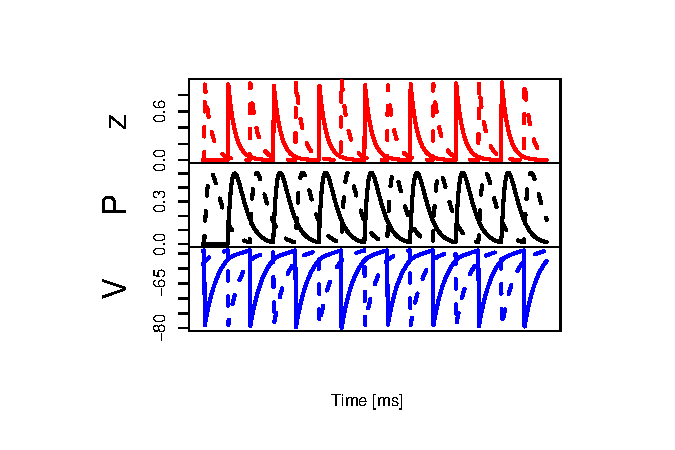
\includegraphics[trim={0 1.8cm 0 1.3cm}, clip, scale=.7]{inhib.pdf}
    \caption{Inhibitory.}
    \label{fig:inhib}
  \end{subfigure}\\
  \begin{subfigure}[t]{.5\textwidth}
    \centering
    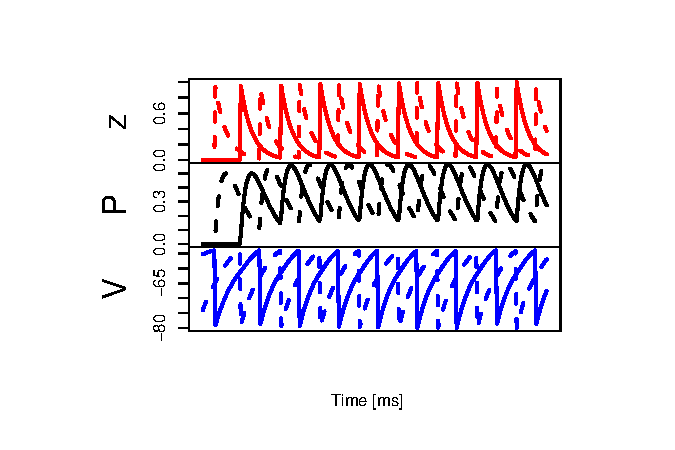
\includegraphics[trim={0 1.8cm 0 1.cm}, clip, scale=.7]{excit.pdf}
    \caption{Excitatory.}
    \label{fig:excit}
  \end{subfigure}%
  \caption{Firing dynamics for a pair of coupled neurons over a range of 500 ms. Note in particular how
1) the neurons appear to lock precisely out of phase from each other, and 2)
that the firing rate for the excitatory neurons is higher than for the
inhibitory ones. Voltage in mV.}
\label{fig:neurons}
\end{figure}

\Cref{fig:inhib,fig:excit} show the two cases with inhibitory and excitatory
neurons respectively. If we compare these rates with the ones shown in the
assignment (and after some digging which reveals that these simulations in fact use a
$P_{max}$ of 1.0), we indeed achieve the correct firing rates. 

% Taus
When we manipulate the $\tau$ factors, which effectively sets the response time
for $P$ and $z$, we investigate proportions between the two constants in order
to evaluate how this changes the dynamics of the system. \Cref{fig:taus} shows
this investigation, where the network has been simulated until converged with
respect to the phase shift under a precision $10^{-5}$. During these
simulations, $\tau_m$ is held constant at 10~ms, whereafter $\tau_s$ takes on
values of powers of two of $\tau_m$. 
\begin{figure}[H]
  \centering
  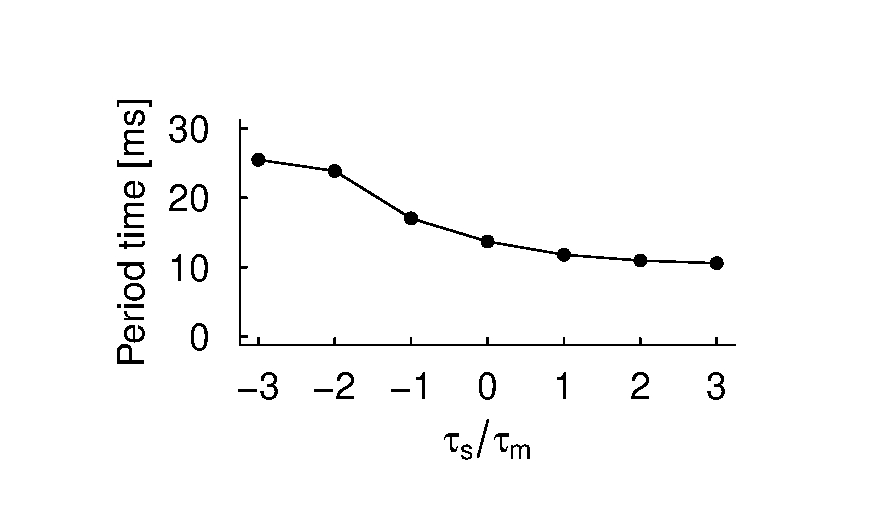
\includegraphics[trim={0 1cm 0 1.cm}, clip, scale=.55]{taus}
  \caption{Dependence of firing rate, or period time, on the proportion
  between the two response factors. The horizontal axis is given in powers
of two, i.e.\ labelling is according to $1 := 2^1, 2 := 2^2$ and so forth.}
  \label{fig:taus}
\end{figure}

% Convergence and stability
\begin{figure}[H]
  \centering
  \begin{subfigure}[t]{.5\textwidth}
    \centering
    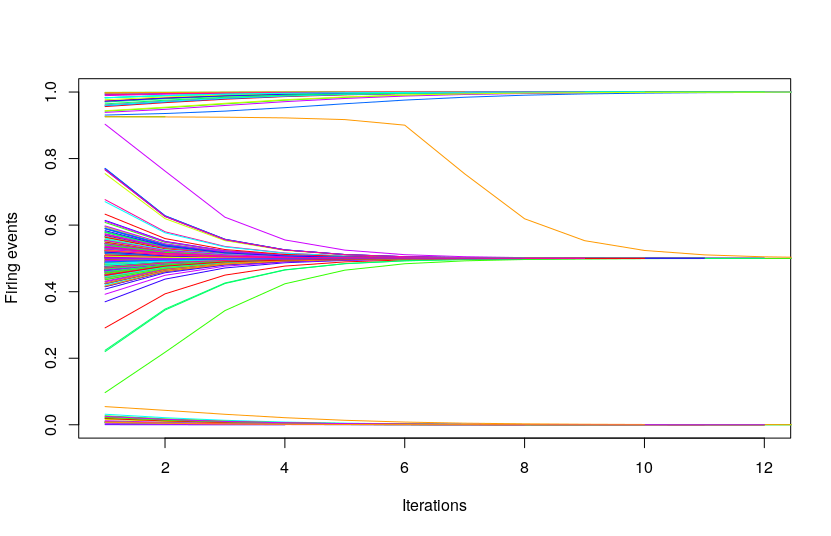
\includegraphics[trim={2.5cm 2.7cm 4cm 2.25cm}, clip,scale=.35]{phase_shift_inhib.png}
    \caption{Inhibitory.}
    \label{fig:inhib_all}
  \end{subfigure}\\
  \begin{subfigure}[t]{.5\textwidth}
    \centering
    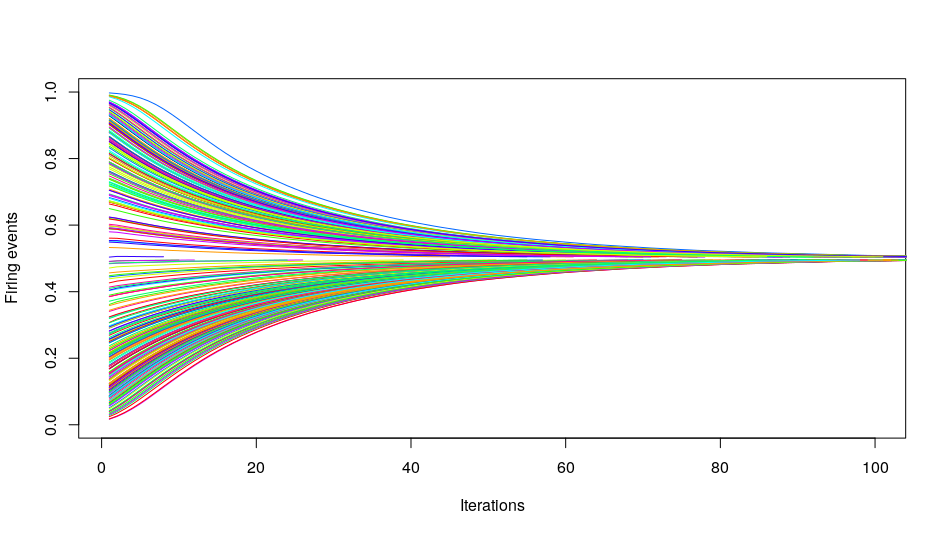
\includegraphics[trim={2.5cm 2.7cm 4cm 2.25cm}, clip,scale=.3]{phase_shift_excit.png}
    \caption{Excitatory.}
    \label{fig:excit_all}
  \end{subfigure}%
  \caption{Phase diagram for the phase shift over the course of 300 simulations.
  The vertical axis shows the fractional phase shift of the period time for one of
the neurons, i.e.\ a value in the range $\left[ 0, 1 \right]$. Note also that
this axis is toroidal, such that a value of 1.0 is functionally equivalent to a
value of 0. The horizontal axis shows the number of firing events. In other words, the trajectories with a less
steep slope converge more slowly. Notably, the excitatory network is more prone
to lock completely out of phase, whereas the inhibitory net is more resilient to
smaller changes.}
\label{fig:comparison}
\end{figure}

As \cref{fig:inhib_all,fig:excit_all} show, the dynamics of the network highly
depened on the interaction between the neurons. If the neurons are excitatory,
for example, the neurons are prone to fire completely out of sync after a long
enough time as passed. When the interaction instead is inhibitory, the neurons
can lock together and fire in synchrony, also if the values are somewhat
deviating initially. However, and as not shown in this figure, the excitatory
neurons can also fire together given that the initial phase shift is not too
large. The boundary for when this locking effect occurs is not easily quantified,
as it depends on the time required for a firing event from the initial
voltages, and not only on the relative difference between them. Still, at a
value of -80 mV for one neuron, a difference of circa 3 mV appears to be the
limit for locking in phase. Under excitatory circumstances, the tolerance is instead
on the order of 0.1.

% Changing the value of E_v
Changing the value of the interaction strength appears to in some cases
destabilize the system. At some positive values of $E_S$, the system seemingly
breaks and stabilizes at a phase shift fraction in neither the vicinity of
$1.0$ nor $0.5$. In other words, there appears to a change in the reachable
attractors given another configuration of parameters.

% Stochastic simulations?
\begin{figure}[H]
  \centering
  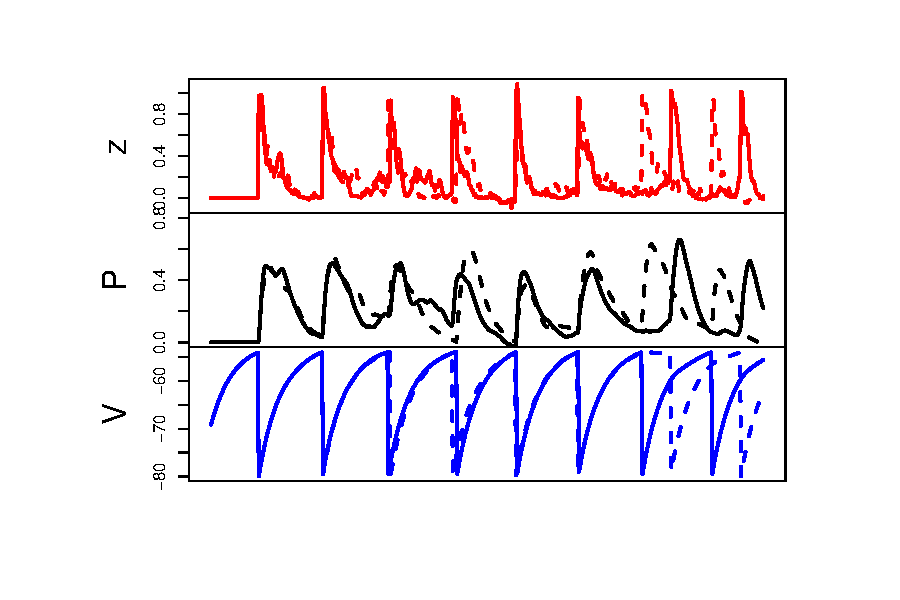
\includegraphics[trim={0 1cm 0 1.cm}, clip, scale=.55]{stochastic}
  \caption{Stochastic simulation of the above dynamics, using a noise reducing factor of
  $\sigma = 3$. Note how in voltage-space the neurons lock and release due to
the noise.}
  \label{fig:stochastic}
\end{figure}
When we simulate the dynamics with noise included, we see the expected
behaviour, namely that the neurons are able to lock into phase with each other,
and subsequently break this lock due to inherent noise in the gating variable.
This can be seen in the latter parts of \cref{fig:stochastic}, where the two
attractors alternatingly are favoured.

\subsection*{Hopfield network}
For our Hopfield network, we investigate various aspects of performance, such as
the ability to recall patterns and the effects of weight-loss. We represent our
nodes as vectors of length 100, where each individual node can take values
$s \in \left\{ -1,1 \right\}$. For training, we use two approaches, namely the
Hebbian training rule, as well as Storkey training, and assess the features of
these two approaches. Whenever the statistical certainty in our results is
shown, it is done so as the standard error of the mean, using 10 simulations per
such investigation.

We measure storage capacity by inputting the stored patterns and iterating the network
until convergence, using an asynchronous and randomly updating rule for the neurons.
If the recovered minimum indeed corresponds to the right pattern, we consider it a
success. 

As a safety-check, we note that the energy is steadily decreasing in all of our
implementations, assuring us of a viable implementation. Also visual analysis of
the patterns stored and retrieved support this (data not shown in either case).

\begin{figure}[H]
  \centering
  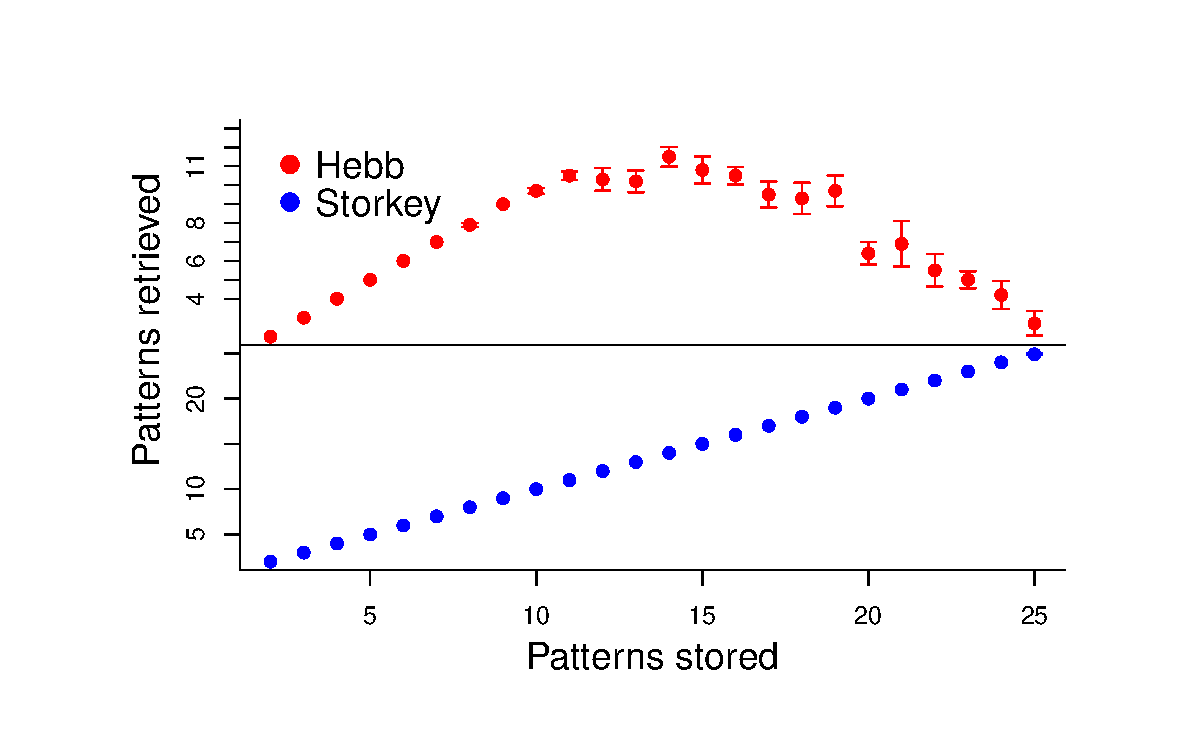
\includegraphics[trim={0 1cm 0 1.cm}, clip, scale=.4]{storage}
  \caption{Storage!}
  \label{fig:storage}
\end{figure}

Using our definition of capacity, the Hebbian net is able to quite successfully
store circa 12.5 patterns in a 100 node network on average, as
\cref{fig:storage} shows, as well as 13 patterns in maximum. This corresponds
well to the theoretical maximum, which would be 13.8 patterns for 100 nodes.
However, this assumes a completely uniform distribution of state values, which
is not the case in our randomly generated patterns. In the Storkey version, we
are able to retrieve far more patterns due to the locality adjustments in the
algorithm. Due to limitation in time, we are however not able to retrieve a
maximum number of stored patterns with our way of measuring this.

% Fraction ones
\begin{figure}[H]
  \centering
  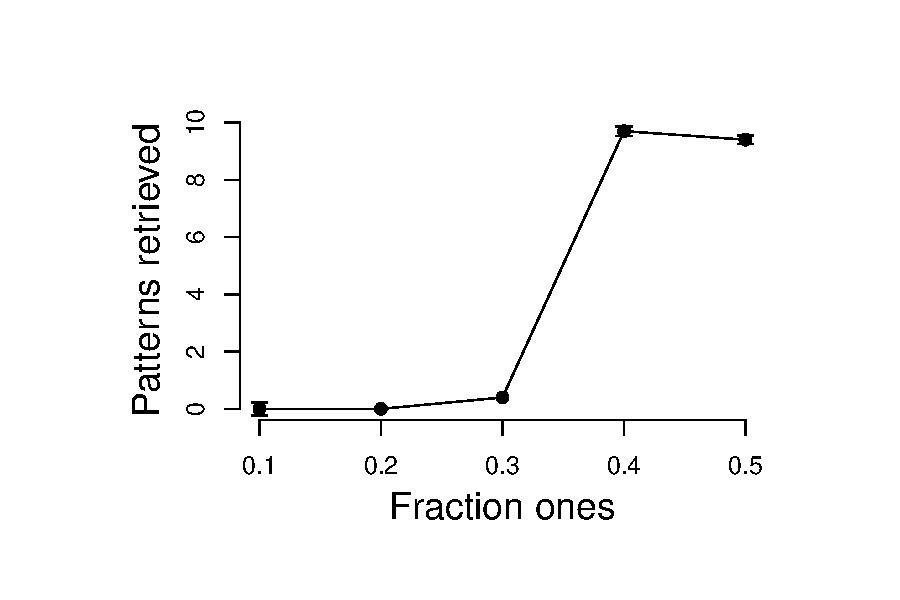
\includegraphics[trim={0 1cm 0 1.cm}, clip, scale=.5]{fraction_ones}
  \caption{A network with 10 patterns stored, and denoted number of bits in the
  patterns set to ones. For skewed sparseness, the network drastically becomes
unable to retrieve the stored patterns.}
  \label{fig:fraction_ones}
\end{figure}

When we change the sparseness in our patterns, the ability to retrieve patterns
clearly changes, which \cref{fig:fraction_ones} indicates. Some variations in
the fraction bits set to either value appears to be managable for the net, but
larger variations struggle significantly, with good results only within the
range of 40-60~\% sparseness. This ought to be due to the high overlap in
the number of bits between the patterns, i.e.\ high correlation, which makes the
network unable to converge towards the correct one. 

\begin{figure}[H]
  \centering
  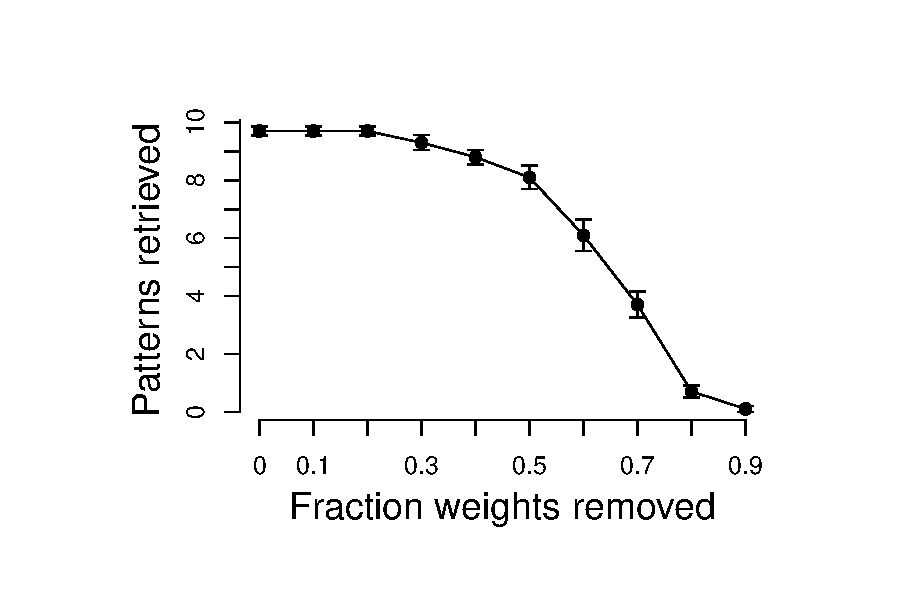
\includegraphics[trim={0 1cm 0 1.cm}, clip, scale=.5]{weights_removed}
  \caption{Network with 10 patterns stored, exposed to removal of a denoted
  fraction of weights. Also with a fairly significant loss of weights, the
network is still able to retrieve most or all patterns.}
  \label{fig:weights_removed}
\end{figure}

In removing weights from the network, we see in \cref{fig:weights_removed} that
for up to 30~\% weights removed, most patterns are still found. It is likely
that also the Stokey net would perform at least similarly, and presumably
better, due to the neighbourhood aspect of the weights, i.e. such that a
neighbourhood can replace the functionality of a single weight in the Hebbian
countervariant. However, due to time constraints, we are unable to show this. 

\section*{Acknowledgements}
Many thanks to my very good friend Julian Melgar for no particular reason. Also
to I\~{n}igo, since he asked for it.

\end{multicols*}
\lstinputlisting{../hop_save.R}
\lstinputlisting{../solver_save.R}


\end{document}
